%!TEX encoding=UTF-8 Unicode
\documentclass[xcolor={usenames,dvipsnames}]{beamer}

%=========================Language and encoding ==============================

\usepackage[utf8]{inputenc}
\usepackage[english]{babel}
\usepackage[T1]{fontenc}
% Fix size errors due to T1 in bbl file
\usepackage{fix-cm}
%=============================================================================

%========================= Todo notes  =======================================

\usepackage{todonotes}
\presetkeys{todonotes}{inline}{}

%=============================================================================

%========================= Figures ===========================================

\usepackage{graphicx} % support the \includegraphics command and options
\graphicspath{ {./img/} }
%\usepackage{tikz}
\usepackage{epstopdf}
\usepackage{booktabs}
\usepackage{multirow}
%\usepackage{subcaption}

%=============================================================================

%=============================================================================

%========================= Hyperref ==========================================

\usepackage{hyperref}
\hypersetup{
    hyperindex=true, %ajoute des liens dans les index.
    colorlinks=false, %colorise les liens
    breaklinks=true, %permet le retour à la ligne dans les liens trop longs
    urlcolor= blue, %couleur des hyperliens
    linkcolor= black, %couleur des liens internes
bookmarksopen=true,}

%=============================================================================

%========================= Other useful includes =============================

\usepackage{ifthen}
\usepackage[absolute,overlay]{textpos} %to set some blocks position
%=============================================================================

%========================= Beamer theme =====================================

%Stuff for printable version
\mode<handout>{
    \usetheme{default}
    \setbeamercolor{background canvas}{bg=black!5}
    \pgfpagesuselayout{4 on 1}[a4paper,landscape,border shrink=2.5mm]
}

\usetheme{AntibesCompact}

\newcommand{\alertitem}{\item<+-|alert@+->}

%=============================================================================

%========================= Title frame  ======================================
\title[]{Analyzing an application memory behavior}
\author[David Beniamine]{\underline{David Beniamine} \and Guillaume Huard \and Bruno
Raffin}
\institute[MOAIS]{
    
\includegraphics[width=.32\textwidth]{img/logoUJF.jpg}
    \qquad
    \qquad
    
\includegraphics[width=.15\textwidth]{img/LIG_coul.jpg}
    \\
    \hspace{50pt}
    
\includegraphics[width=.22\textwidth]{img/inria.jpg}
    \qquad
    
\includegraphics[width=.4\textwidth]{img/moais.png}
}
%=============================================================================

\begin{document}
%========================= Title and outlines ================================
\begin{frame}{}
    \titlepage
\end{frame}

\newboolean{sectiontoc}
\setboolean{sectiontoc}{true} % default to true

\AtBeginSection[]
{
    \ifthenelse{\boolean{sectiontoc}}{
        \begin{frame}<beamer>
            \frametitle{Outline}
            \tableofcontents[currentsection,currentsubsection]
        \end{frame}
    }
}
\AtBeginSubsection[]
{
    \ifthenelse{\boolean{sectiontoc}}{
        \begin{frame}<beamer>
            \frametitle{Outline}
            \tableofcontents[currentsection,currentsubsection]
        \end{frame}
    }
}

%=============================================================================

%========================= Real presentation =================================
\begin{frame}{Outline}
    \tableofcontents
\end{frame}

\section{Context and motivations}
\begin{frame}{Memory on HPC}
    \begin{itemize}[<+->]
        \item $100$ of CPU cycles per memory access
        \item Cache hierarchy
        \item NUMA machines
        \item GPGPU / Xeon Phi \dots
    \end{itemize}
    \pause
    \begin{exampleblock}{Question}
        How to analyze and optimize memory usage ?
    \end{exampleblock}
\end{frame}

\begin{frame}{Analysis tools}
    \begin{itemize}
        \item Performance counters~\cite{Treibig10LIKWID} 
        \item Vtunes~\cite{Reinders05VTune}
        \item HPCTOOLKIT~\cite{Adhianto10HPCTOOLKIT}
        \item \ldots
    \end{itemize}
    \pause
    \begin{alertblock}{Limits}
            Do not explain memory issues
    \end{alertblock}
\end{frame}
\begin{frame}{Memory oriented tools}
    \begin{itemize}[<+->]
        \item Data and Thread Mapping
            \begin{itemize}
                \item Manual \alert{require knowledge}
                \item  Adaptive~\cite{Diener13CommunicationBased,Levinthal2009}
                    \begin{itemize}
                        \item Collect and use data online
                        \alertitem Cannot change memory pattern
                    \end{itemize}
            \end{itemize}
        \item Existing memory
            profilers~\cite{Lachaize12MemProf,Gimenez14Dissecting,Liu14Tool}
            \begin{itemize}
                \item Based on CPU counters \alert{indirect information}
                \item Sampling (IBS/PEBS etc.) \alert{not complete}
                \item \alert{Focus on particular events} (remote accesses,
                    cache miss etc.)
            \end{itemize}
    \end{itemize}
\end{frame}
\section{Memory Analysis}
\subsection{Tabarnac}
\subsubsection*{Design}
\begin{frame}{Goal}
    \begin{itemize}[<+->]
        \item NUMA oriented
        \item Data structure centred
        \item Memory access balance 
            \begin{itemize}
                \item Between threads
                \item Between pages
            \end{itemize}
        \item Sharing pattern
    \end{itemize}
\end{frame}

\begin{frame}{Main principles}
    \begin{itemize}[<+->]
        \item Pin instrumentation
            \begin{itemize}
                \item Counters Pages / thread
            \end{itemize}
        \item Data oriented visualization
        \item Simple yet meaning full plots
            \begin{itemize}
                \item Structure size
                \item Number of read/write per structure
                \alertitem Accesses distribution by on each structure
                \alertitem First touch distribution by on each structure
            \end{itemize}
        \item Easy to use interface with explanations for new users
    \end{itemize}
\end{frame}

\subsubsection*{Example}

\begin{frame}{IS accesses distribution}
    \begin{figure}
        \centering
        \vspace{-10pt}
        \alt<1>{
            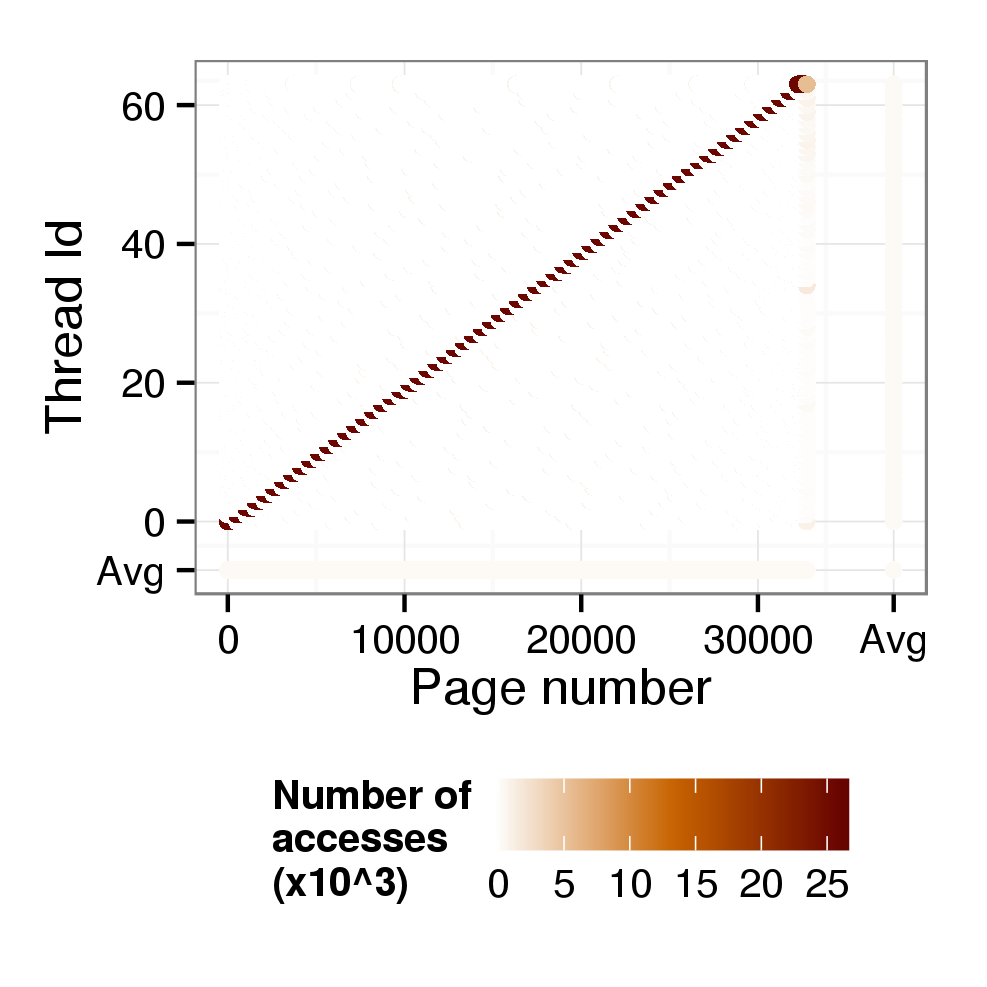
\includegraphics[width=.6\linewidth]{is_b_kba_orig.png}
            \caption{Access distribution on structure key array}
        }{\alt<2>{
            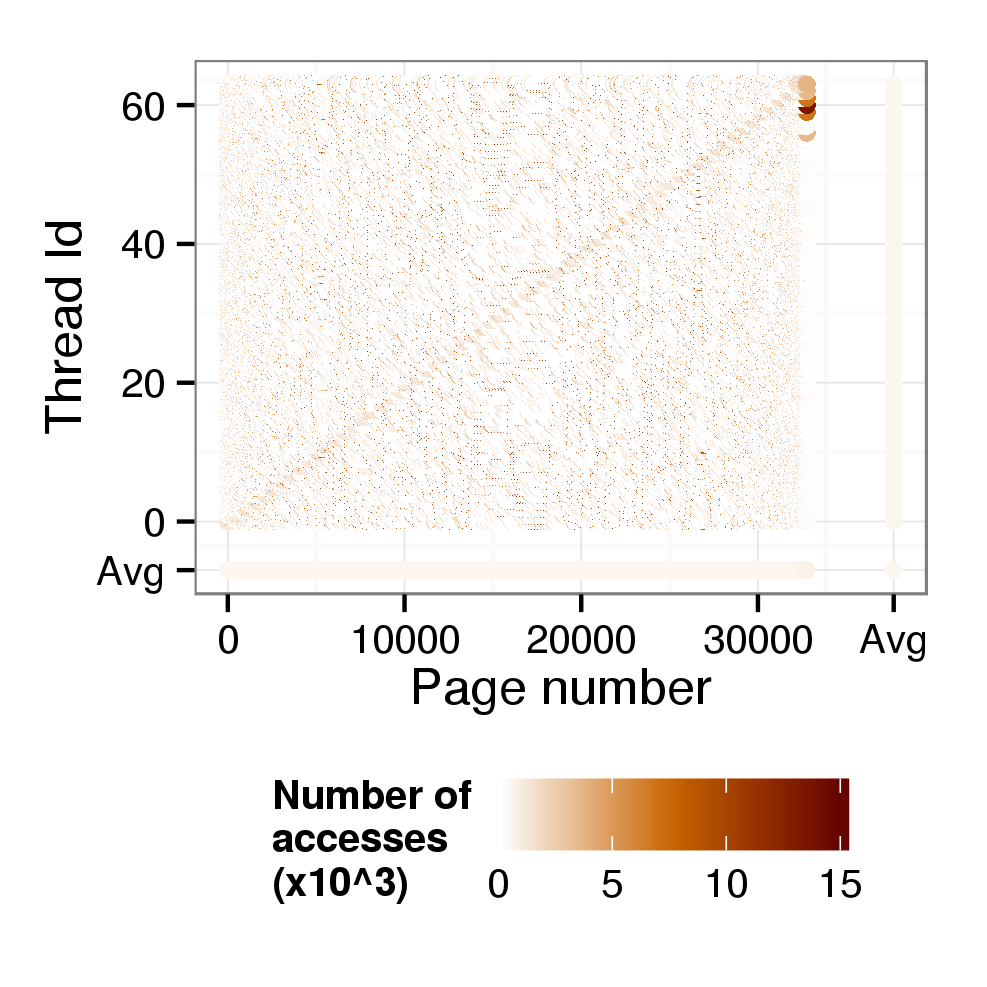
\includegraphics[width=.6\linewidth]{is_b_kb2_orig.png}
            \caption{Access distribution on structure key buff 2}
        }{
            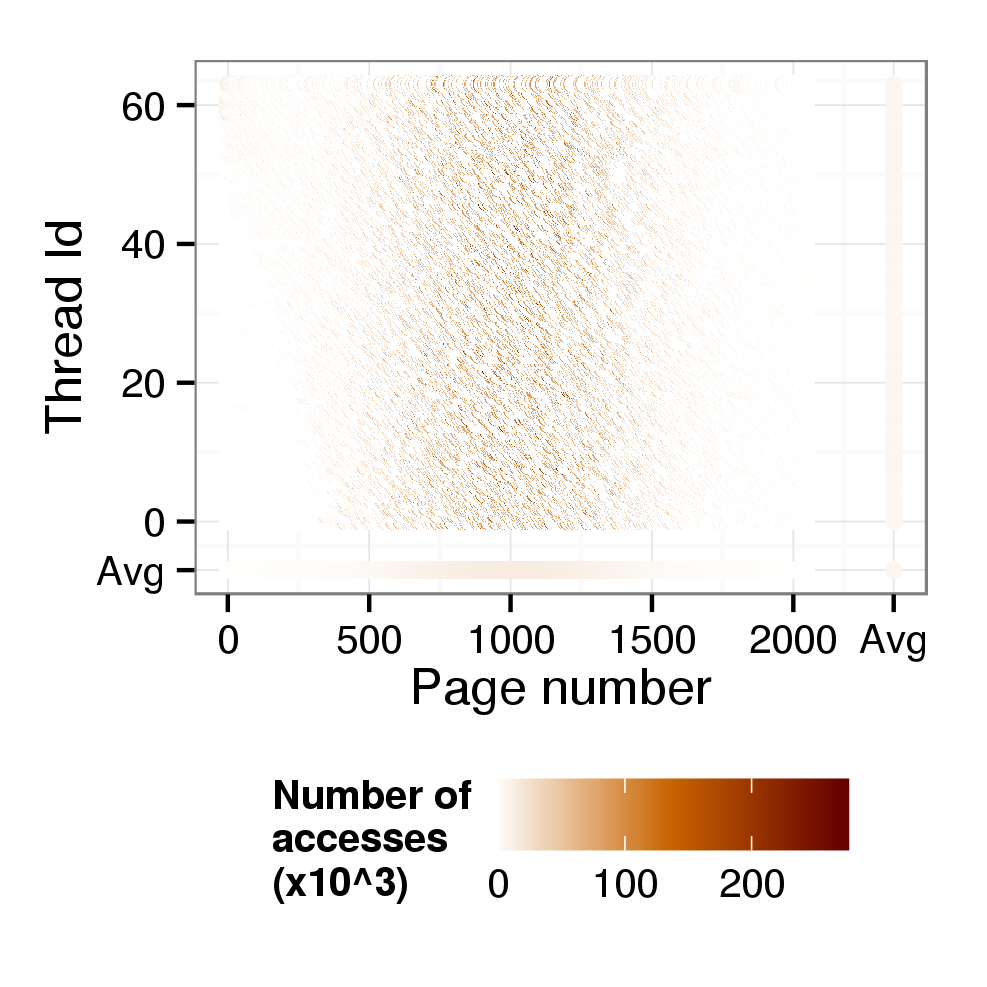
\includegraphics[width=.6\linewidth]{is_b_kb1_orig.png}
            \caption{Access distribution on structure key buff 1}
        }
    }
\end{figure}
\pause
\pause
\end{frame}

\begin{frame}{What to do now ?}
    \begin{exampleblock}{What is happening ?}
        \begin{itemize}
            \item Access to \texttt{kb1} using values from \texttt{kb2}
            \item Values of \texttt{kb2} follows a Gaussian distribution
            \item Dynamic (OpenMp) thread scheduling
        \end{itemize}
    \end{exampleblock}
    \pause
    \begin{alertblock}{How to fix this pattern}
        \begin{itemize}
            \item Split the Gaussian
            \item Cyclic distribution on each side
            \item Give each thread the same amount of memory accesses
        \end{itemize}
    \end{alertblock}
\end{frame}

\begin{frame}{New accesses distribution}
    \begin{figure}
        \centering
        \vspace{-10pt}
        \alt<1>{
            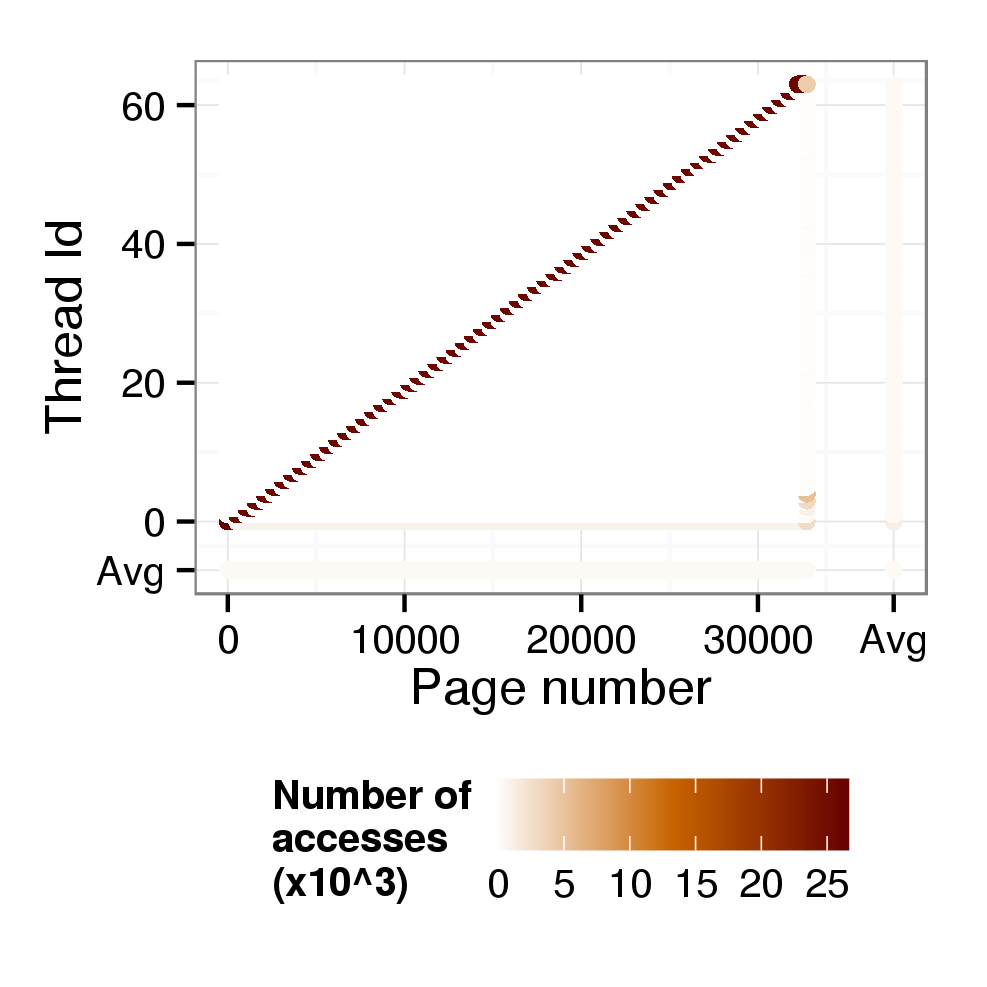
\includegraphics[width=.6\linewidth]{is_b_kba_modif.png}
            \caption{Modified access distribution on structure key array}
        }{\alt<2>{
            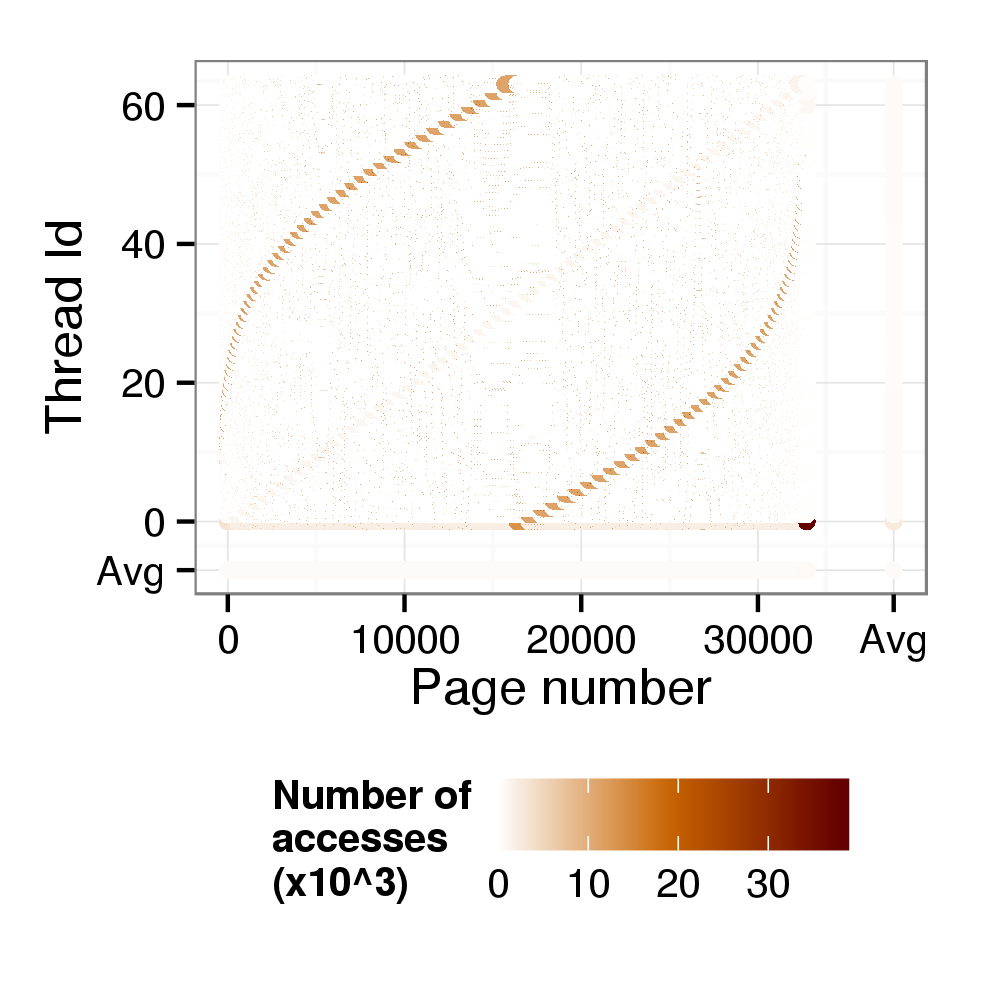
\includegraphics[width=.6\linewidth]{is_b_kb2_modif.png}
            \caption{Modified access distribution on structure key buff 2}
        }{
            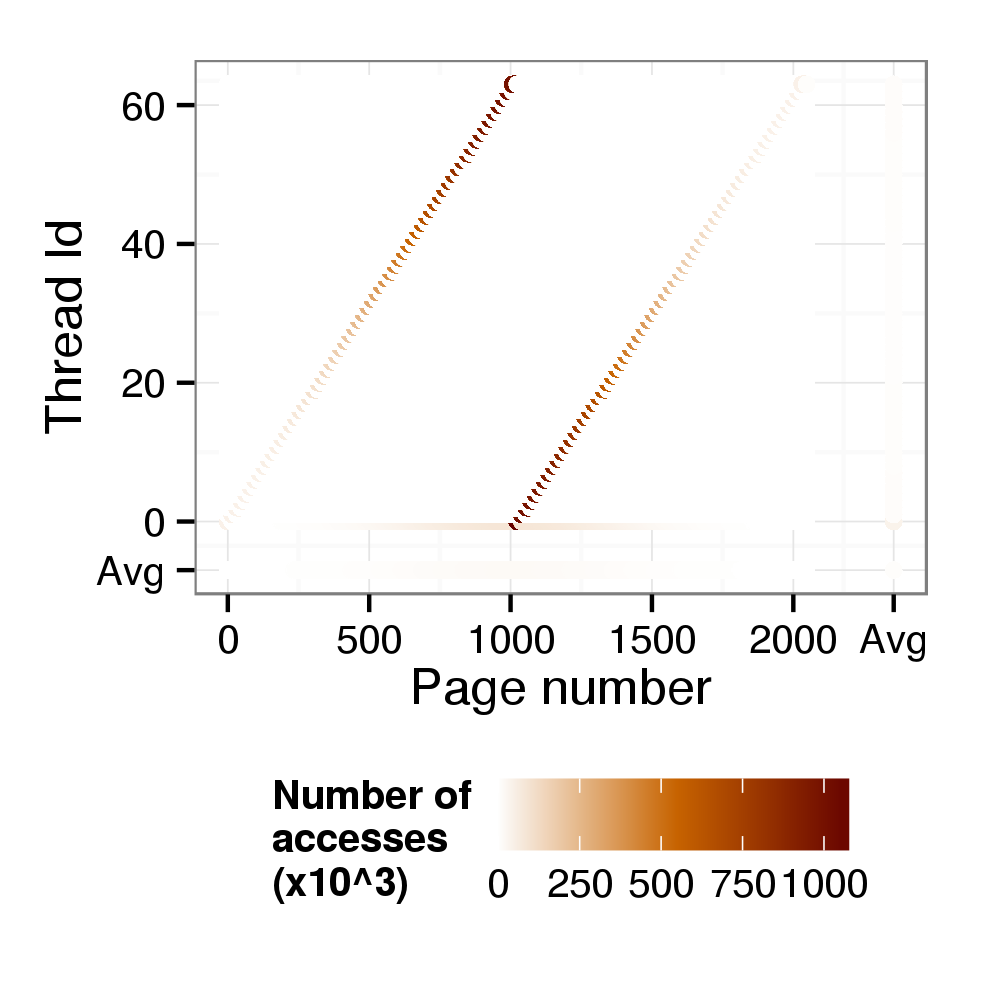
\includegraphics[width=.6\linewidth]{is_b_kb1_modif.png}
            \caption{Modified access distribution on structure key buff 1}
        }
    }
\end{figure}
\pause
\pause
\end{frame}

\begin{frame}{Results}
    \alt<1>{
        \begin{itemize}
            \item Optimization methods
                \begin{itemize}
                    \item Base (OS)
                    \item Numa Balancing (adaptive mapping)
                    \item Interleave (static mapping)
                \end{itemize}
            \item Thread distributions
                \begin{itemize}
                    \item Dynamic (default)
                    \item Cyclic (don't split the loop, unbalanced access)
                    \item Cyclic-split (described earlier + manual mapping)
                \end{itemize}
        \end{itemize}
    }{
        \begin{figure}[]
            \centering
            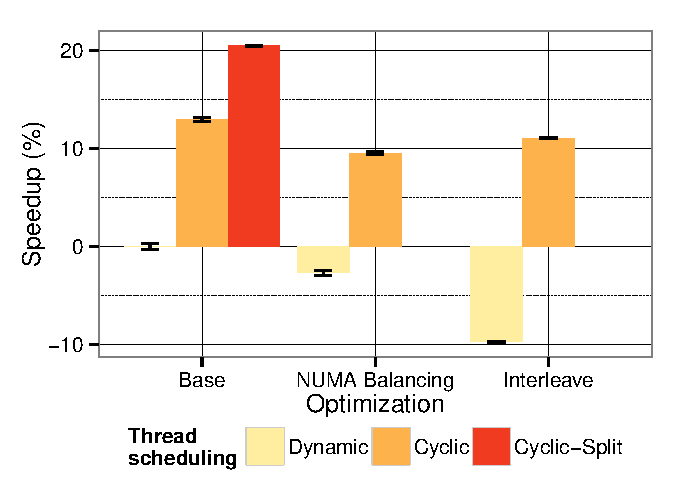
\includegraphics[width=.7\linewidth]{is_exectime.pdf}
            \caption{Evaluation of the modified code}
        \end{figure}
    }
    \pause
\end{frame}

\subsection{Moca}

\subsubsection*{Design}

\begin{frame}{Goal}
    \begin{itemize}[<+->]
        \item Accesses distribution
        \item Thread Sharing
        \item CPU Location
        \alertitem Temporal evolution
        \alertitem Superset of the pages
        \item Detail at the byte granularity
        \item Reasonable overhead
        \alertitem Portability
    \end{itemize}
\end{frame}

\begin{frame}{Main principles}
    \begin{itemize}[<+->]
        \alertitem Page fault interception
        \item False page fault (inspired by~\cite{Diener12Using})
        \item Linux kernel module
        \item Temporary flush data to disc
    \end{itemize}
\end{frame}

\subsubsection*{Evaluation}

\begin{frame}{Overhead on NPB}
    \begin{figure}[]
        \centering
        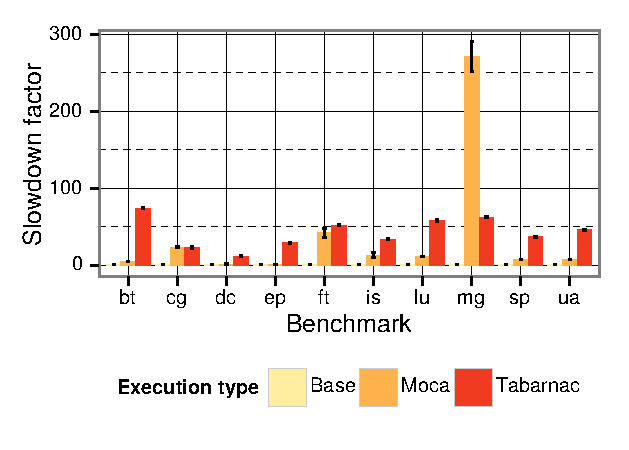
\includegraphics[width=.7\linewidth]{moca_overhead_nas.pdf}
        \caption{Overhead of Moca compared to Tabarnac on the NPB, edel
        cluster}
    \end{figure}
\end{frame}

\begin{frame}{Unique addresses intercepted}
    \begin{figure}[]
        \centering
        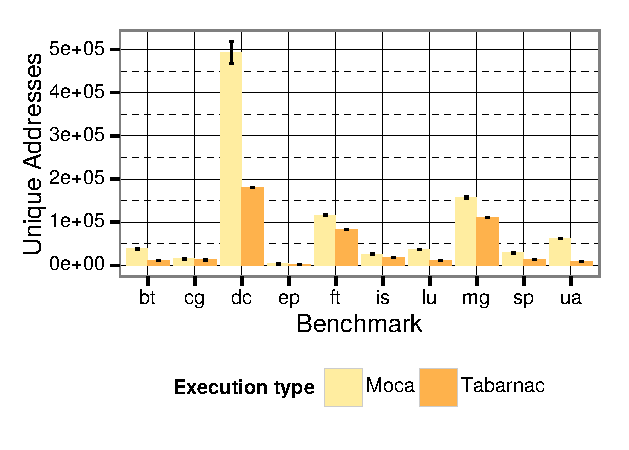
\includegraphics[width=.7\linewidth]{moca_addresses_nas.pdf}
        \caption{Number of addresses captured on Moca compared to Tabarnac on the NPB, edel
        cluster}
    \end{figure}
\end{frame}
\subsubsection*{Visualization}

\begin{frame}{Design}
    \begin{itemize}
        \item Based on Ocelotl~\cite{Dosimont14Trace}
        \item Aggregate data to identify anomalies
        \item Cartography view of the memory accesses
        \item global / by thread visualization
    \end{itemize}
\end{frame}

\begin{frame}{Example}
    \begin{figure}[]
        \centering
        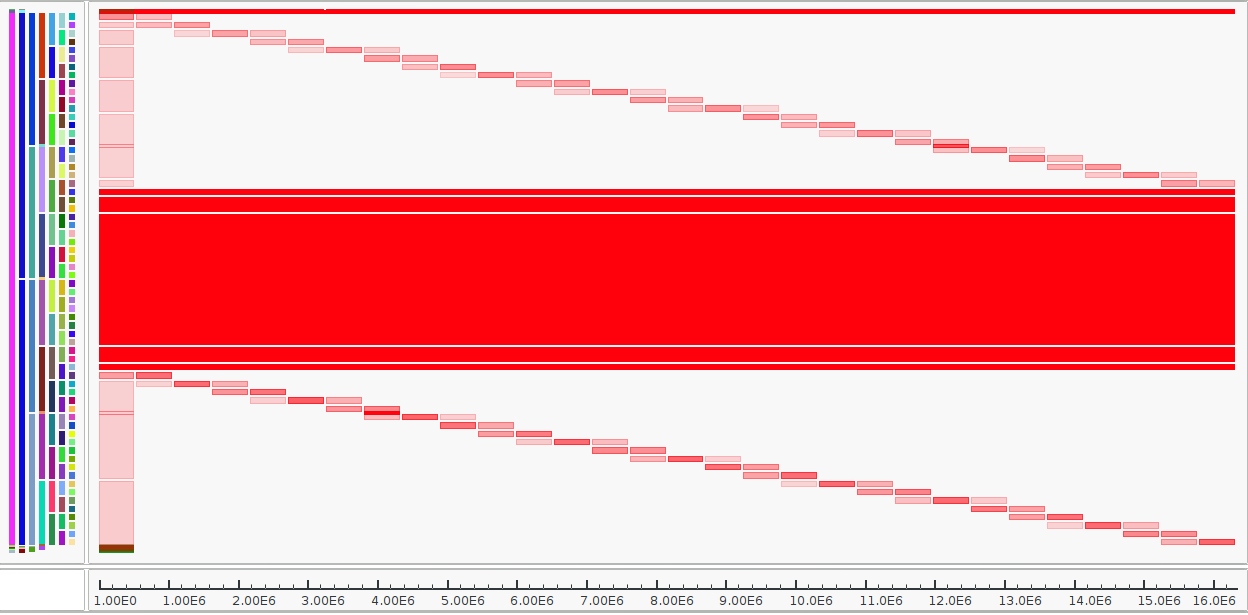
\includegraphics[width=\linewidth]{ocelotl.png}
        \caption{Example visualisation of Moca with Ocelotl}
    \end{figure}
\end{frame}

\section{Conclusions and perspectives}
\begin{frame}{Conclusion}
    \begin{exampleblock}{Using efficiently memory is hard}
        How can we understand an applications memory behavior ?
    \end{exampleblock}
    \pause
    \begin{block}{Tabarnac (joint work UFRGS / UJF, accepted at VPA'15)}
        \begin{itemize}
            \item Global view
            \item NUMA oriented
            \item Simple to use
            \item No temporal informations
        \end{itemize}
    \end{block}
    \pause
    \begin{alertblock}{Moca (submitted at IPDPS'15)}
        \begin{itemize}
            \item Extremely complete trace
            \item Reasonable overhead
            \item Temporal informations
        \end{itemize}
    \end{alertblock}
\end{frame}

\newcounter{finalframe}
\setcounter{finalframe}{\value{framenumber}}
%Last numbered frame go here

\begin{frame}{Future work}
    \begin{block}{Study case and Optimization}
        Analyse and study more real applications
    \end{block}
    \pause
    \begin{alertblock}{Visualization and analysis}
        \begin{itemize}[<+->]
            \item Moca visualization is a prototype.
            \item Automatic analysis posible ?
            \item Compute metrics / grade memory patterns
        \end{itemize}
    \end{alertblock}
\end{frame}
%=============================================================================

%=============================================================================
%Uncomment next lines for uncounted backup slides & biblio
\section*{Bibliography}
%
\bibliographystyle{apalike}
\bibliography{biblio}

%========================= Backup slides =====================================
\section*{Hidden slides}
%put this line before each frame

\setcounter{framenumber}{\value{finalframe}}
\begin{frame}{Moca full visualization}
    \begin{figure}
        \centering
        \alt<1>{
            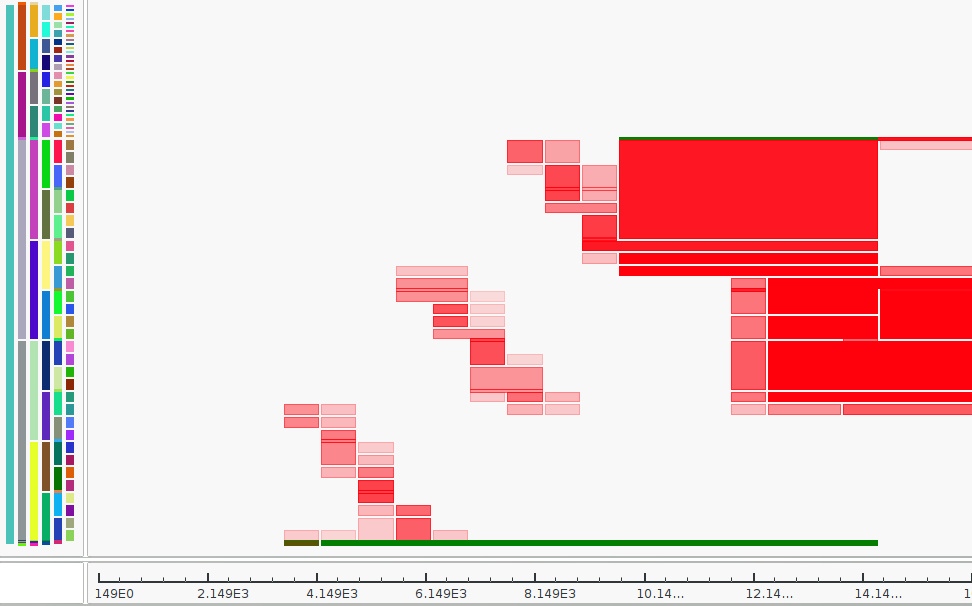
\includegraphics[width=.8\linewidth]{moca_init.png}
            \caption{Moca trace, zoom on intialisation}
        }{
            \alt<2>{
                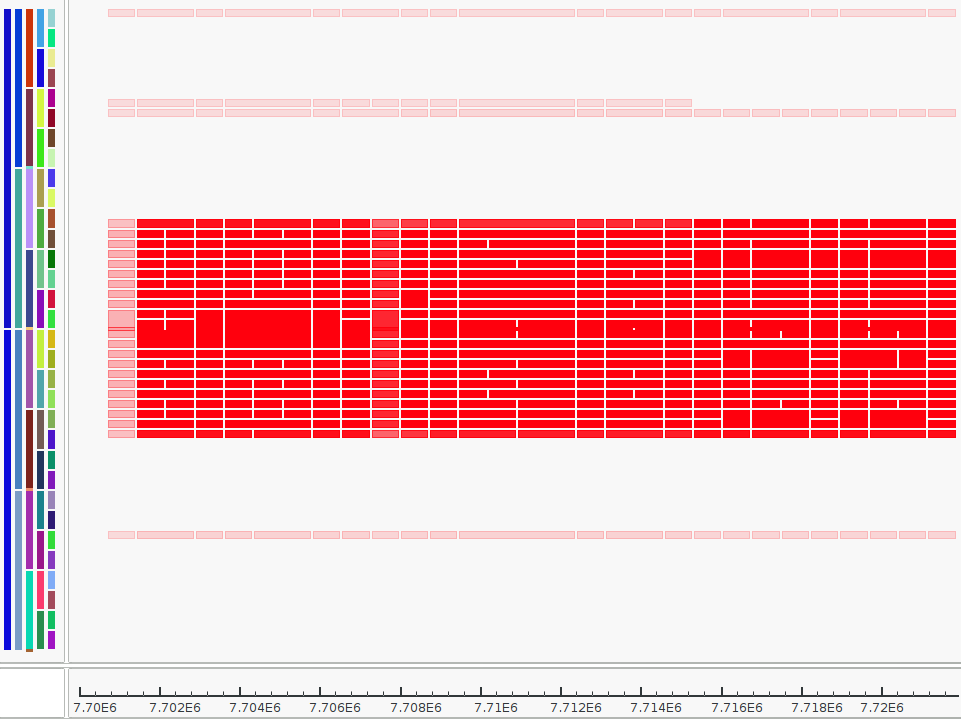
\includegraphics[width=.8\linewidth]{moca_zoom.png}
                \caption{Moca trace zoomed}
            }{
                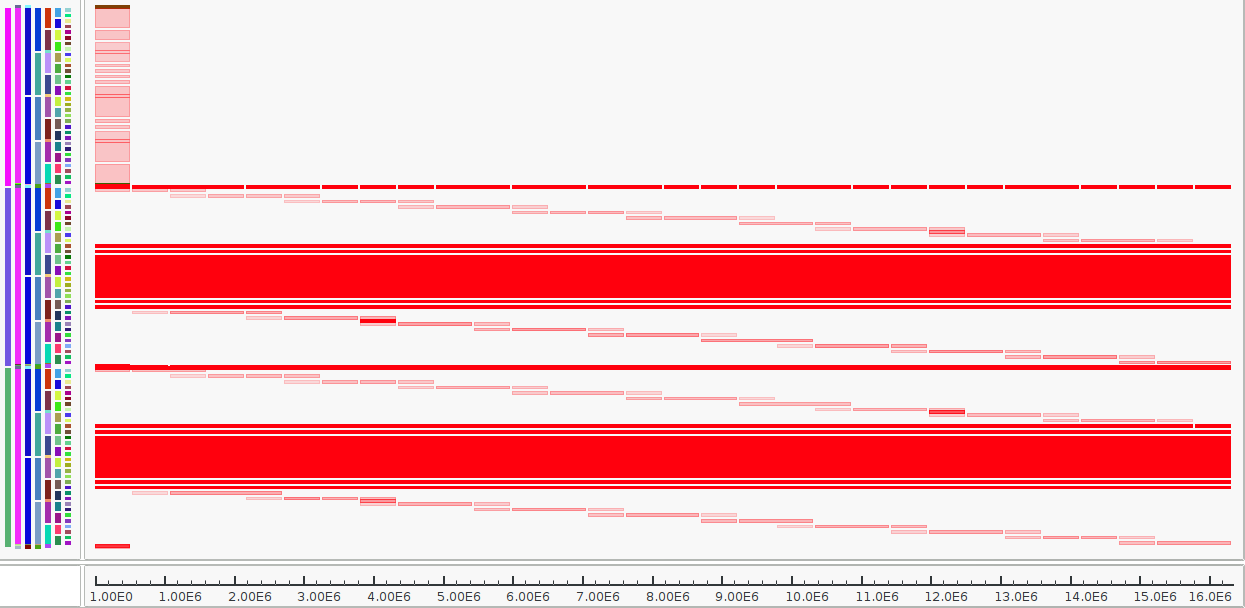
\includegraphics[width=.8\linewidth]{moca_thread.png}
                \caption{By thread visualization of Moca trace}
            }
        }
    \end{figure}
    \pause
    \pause
\end{frame}

\setcounter{framenumber}{\value{finalframe}}
\begin{frame}{Tabarnac full visualization}
    \begin{figure}
        \centering
        \vspace{-10pt}
        \alt<1>{
            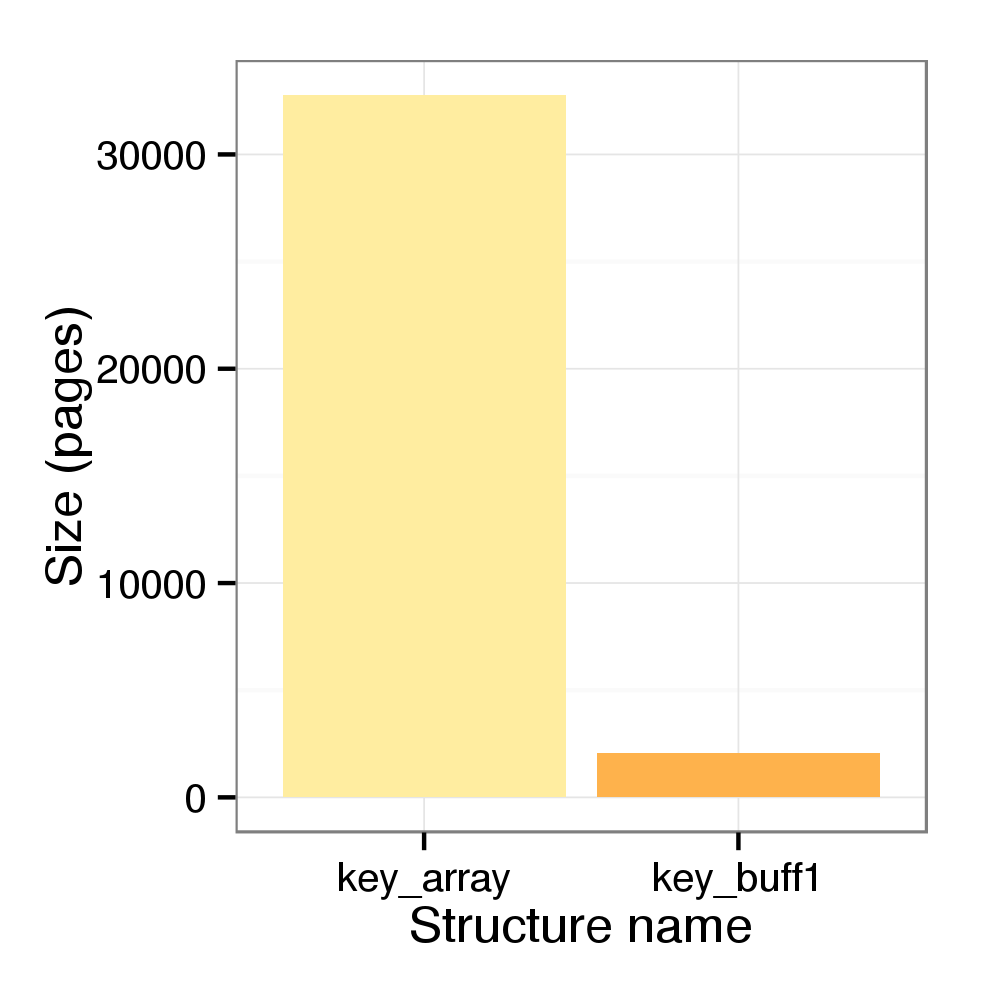
\includegraphics[width=.6\linewidth]{tabarnac_sz.png}
            \caption{Structure sizes}
        }{
            \alt<2>{
                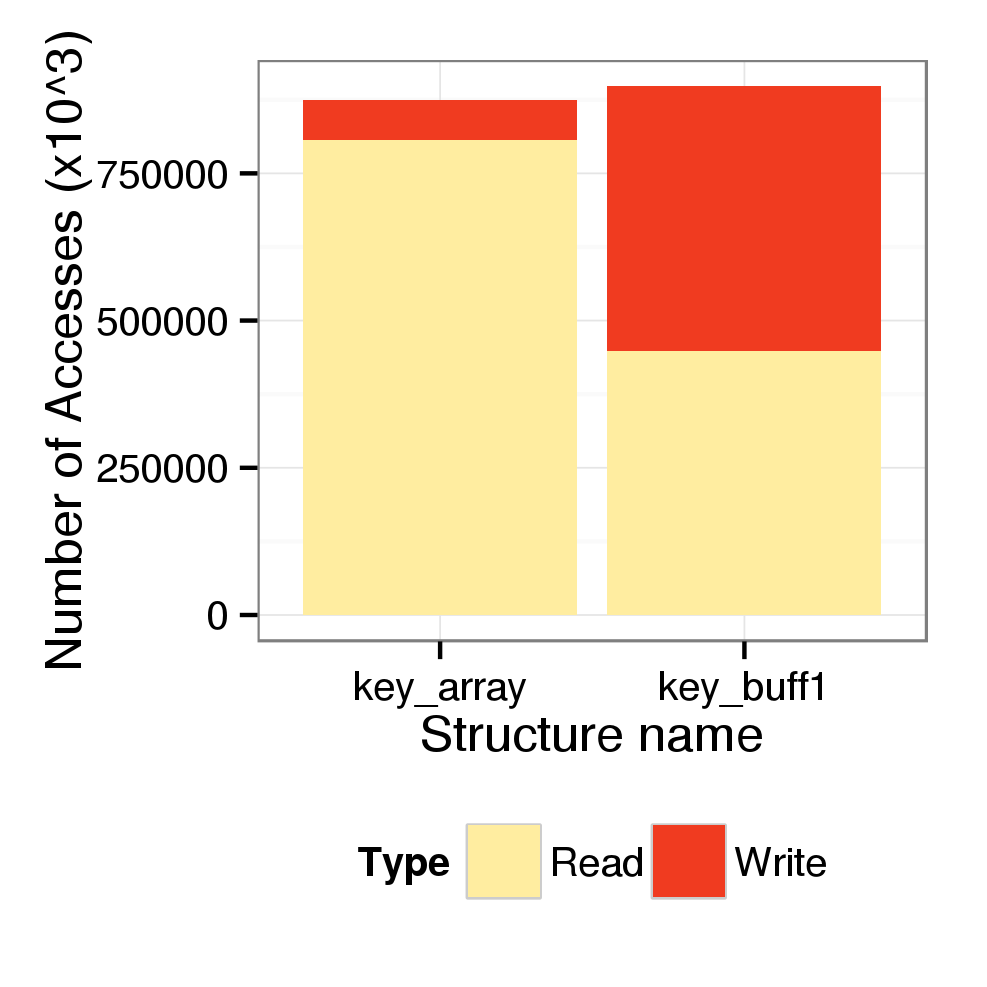
\includegraphics[width=.6\linewidth]{tabarnac_rw.png}
                \caption{Read and writes by structures}
            }{
                \alt<3>{
                    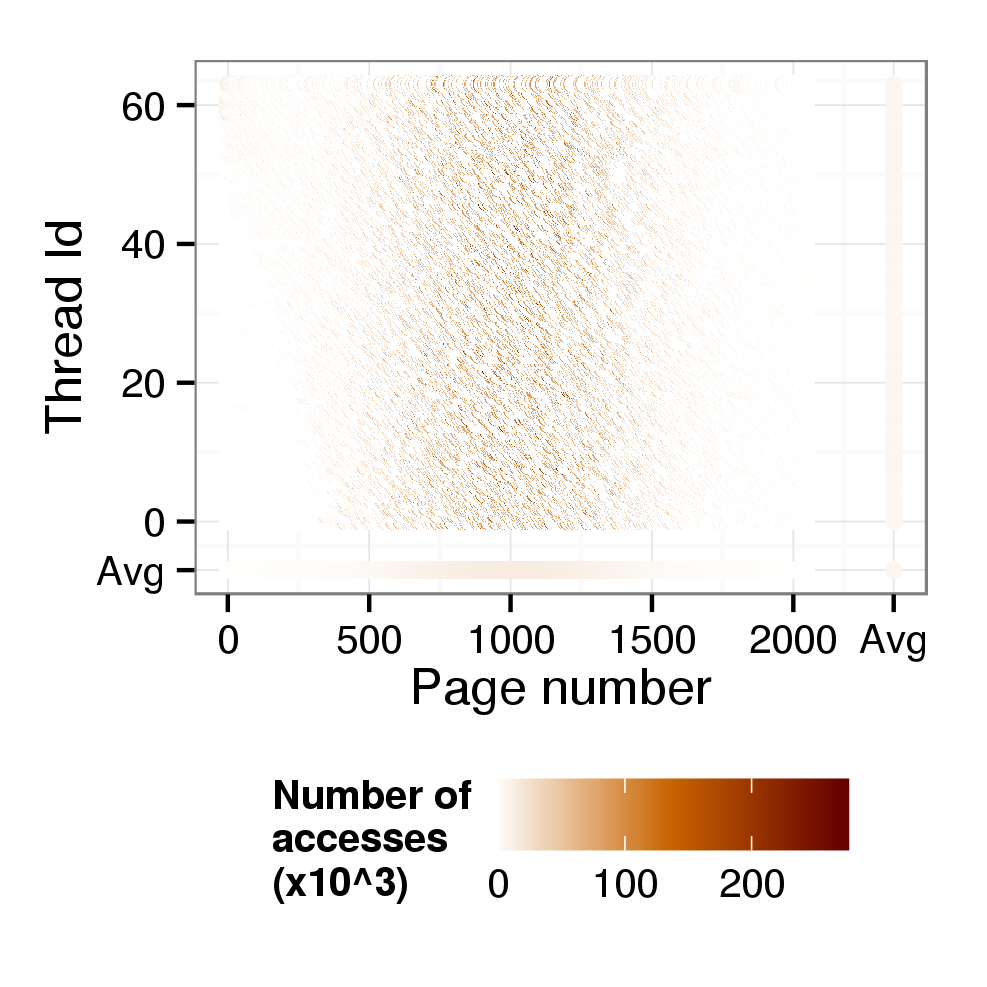
\includegraphics[width=.58\linewidth]{tabarnac_dist.png}
                    \caption{Access distribution}
                }{
                    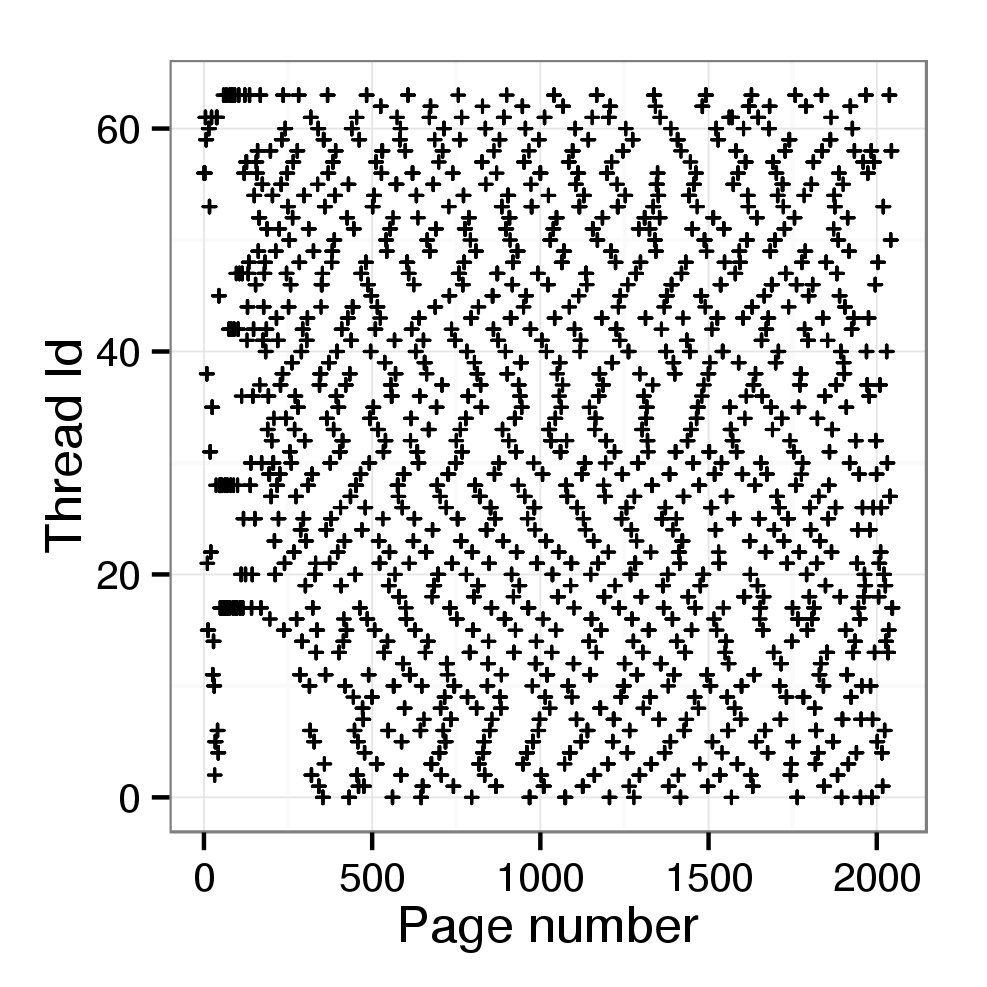
\includegraphics[width=.6\linewidth]{tabarnac_ft.png}
                    \caption{First touch distribution}
                }
            }
        }
    \end{figure}
    \pause
    \pause
    \pause
\end{frame}



\setcounter{framenumber}{\value{finalframe}}
\begin{frame}{Tabarnac Overhead}
    \begin{figure}
        \centering
        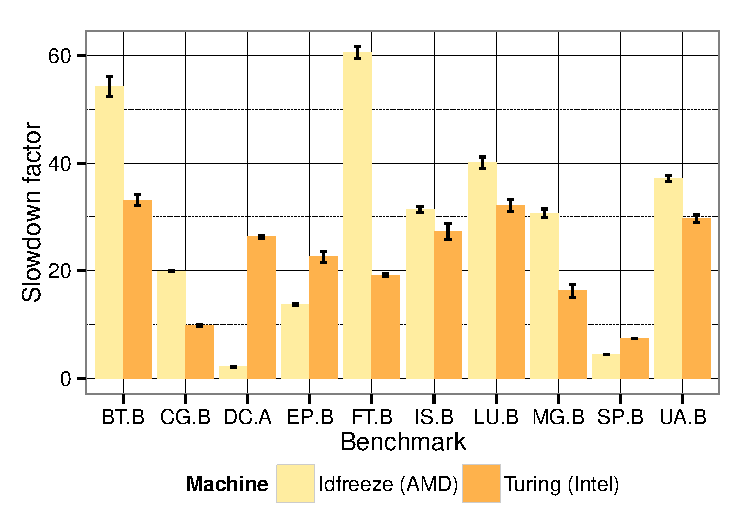
\includegraphics[width=.8\linewidth]{tabarnac_ovh.pdf}
        \caption{Overhead of Tabarnac on the NPB on a 64 cores NUMA machine}
    \end{figure}
\end{frame}

% Tabarnac full vizu
\setcounter{framenumber}{\value{finalframe}}
\begin{frame}{Machines}
    \centering{
    \resizebox{.7\linewidth}{!}
    {
    \begin{tabular}{lp{1.1cm}rrp{1.35cm}p{1.1cm}}
        \toprule
        \multirow{3}{.8cm}{CPU}
        &  & \multicolumn{2}{c}{Vendor} & \multicolumn{2}{c}{Model} \\
        \cmidrule(lr){3-6}
        & \texttt{Turing}  & \multicolumn{2}{c}{Intel} & \multicolumn{2}{c}{Xeon X7550} \\
        & \texttt{Idfreeze} & \multicolumn{2}{c}{AMD} & \multicolumn{2}{c}{Opteron 6174} \\
        & \texttt{Edel} & \multicolumn{2}{c}{Intel} & \multicolumn{2}{c}{Xeon E5520} \\
        \midrule
        \midrule
        \multirow{3}{.8cm}{System totals}
        & & Nodes & Threads & Freq & Memory \\
        \cmidrule(lr){3-6}
        & \texttt{Turing}   & $4$ & $64$ & $2.00$ Ghz & $128$ Gib \\
        & \texttt{Idfreeze} & $8$ & $48$ & $2.20$ Ghz & $256$ Gib\\
        & \texttt{Edel} & $2$ & $4$ &  $2.27$ Ghz & $24$ Gib\\
        \midrule
        \midrule
        \multirow{3}{.8cm}{Per node}
        & & Cores & Threads & L3 Cache & Memory \\
        \cmidrule(lr){3-6}
        & \texttt{Turing}   & $8$ & $16$ & $18$ Mib & $32$ Gib \\
        & \texttt{Idfreeze} & $6$ & $6$  & $12$ Mib & $32$ Gib \\
        & \texttt{Edel} & $4$ & $4$  & $8$ Mib & $12$ Gib \\
        \bottomrule
    \end{tabular}
    }}
\end{frame}
%=============================================================================
\end{document}




